\section{Analysis of the sine modeling  method}
The analysis of the sinus method consists of multiple parts: First the error threshold was computed, which will be used to determine the first absorption dip from each of the change of channels per change of frequency measurements.
Second, the change of channels per change of frequency was computed, choosing one of the dips as reference. 
Third, the actual resonance frequency for each measurement was computed with the relation of the second step of this part of the analysis.
Fourth, the combination of the measured magnetic fields and computed frequencies was used to compute the magnetic momentum of the proton in $^{19}$F and the gyromagnetic ratio of the proton in glycol and hydrogen.
\subsection{Error thresholds}
%  Although two different pure background measurements were recorded, they ended up replaced by the noise recorded during the measurements for the change of channel per change of frequency.
For the error thresholds, one has to take a closer look at the recorded data. The .csv files obtained during the experiment contain the maxima and minima of the curves seen on the oscilloscope. To get a limit which is useful to discriminate the data multiple preparatory steps were necessary: First the absolute values of the differences from two neighbouring background data points were computed and projected to the y axis. A Gaussian curve was fitted to this projection. The maximum of the fitted curve, subtracted from to the mean of the background data used for the projection was the lower error threshold.\par 
In comparison to the out sample or in sample of frequency background, the background during the actual measurement is the most representative, because it was obtained during the exact same conditions as the signal data.
After taking an initial look at the measurements used for the frequency difference per channel difference (as seen in fig. \ref{all_dx}), it was decided that a sufficient amount of background data points can be obtained from these measurements. 
\begin{figure}[h]
	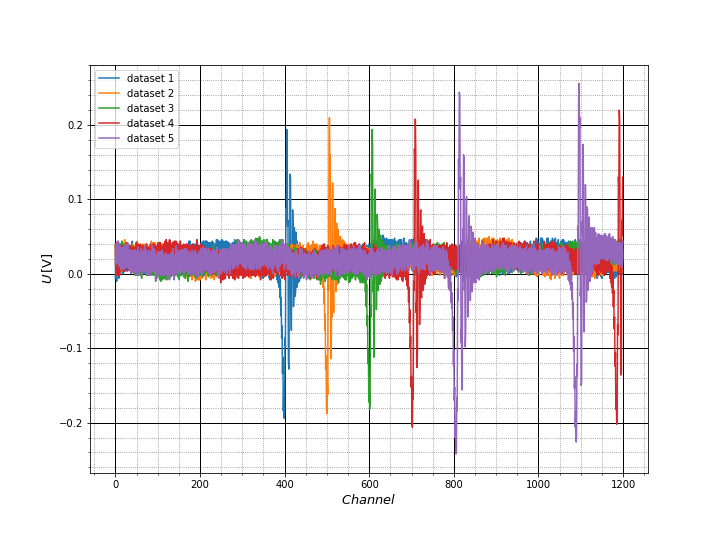
\includegraphics[scale=0.5]{Bild/all_dx.png}
	\centering
	\caption[Plot of all data used for the discriminator determination]{Plot of the measured voltage against the channel of the data points from all five measurements used for the difference in frequency per difference in channel.}
	\label{all_dx}
\end{figure}

After examining the first absorption peak of the first dataset, the parameter to coarsely seperate the background from the absorbtion signals was determined to be $-0.03\,$V. Both can be seen in fig. \ref{absorbtionpeak}. All values up to the tenth value underneath this threshold are considered as background signal.\par
\begin{figure}[h]
	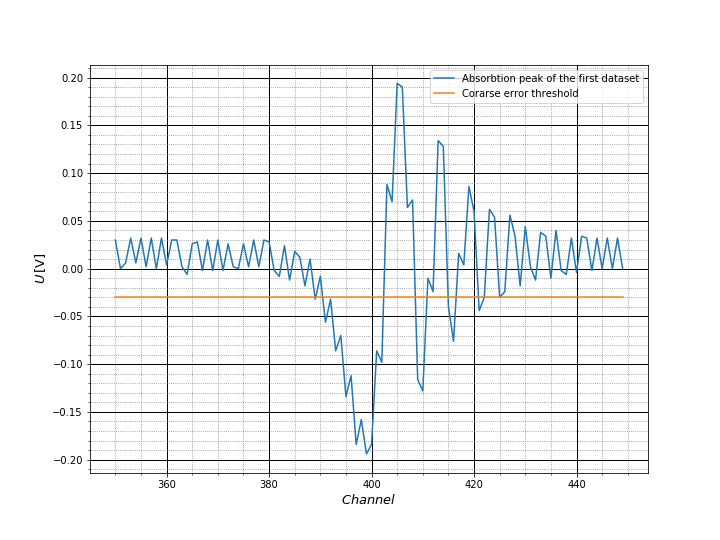
\includegraphics[scale=0.5]{Bild/peak_first_single.png}
	\centering
	\caption[Plot of an absorption peak]{Plot of the measured voltage against the channel of the absorption peak of the first measurement taken for the frequency change channel change ration measurement series. Also seen is the coarse error threshold of $-0.03\,$V.}
	\label{absorbtionpeak}
\end{figure}

All of these values can be seen in fig. \ref{all_err}. Now, the absolute difference between two neighbouring points was computed, which can be seen in fig. \ref{err_abs}. It is clearly visible, that all the data points in fig. \ref{all_err} and absolute differences in fig. \ref{err_abs} come in discrete levels. The reason behind this is the limited resolution of the analogue digital converter in the oscilloscope, which represents the values as binary numbers of a certain length, allowing only discrete voltage levels to be displayed. \par
These discrete levels result in zeros in the projection of the values to the y axis, which were not considered for the fit of the Gaussian curve. 
